% ----------------------------------------------------------------------------------------
% This contains all the content under Part: System Architecture
% ----------------------------------------------------------------------------------------
\part{System Architecture}
\chapter{A Generic Application Processor}
\label{chap:genericAP}
	\begin{figure}[h]
	\centering
	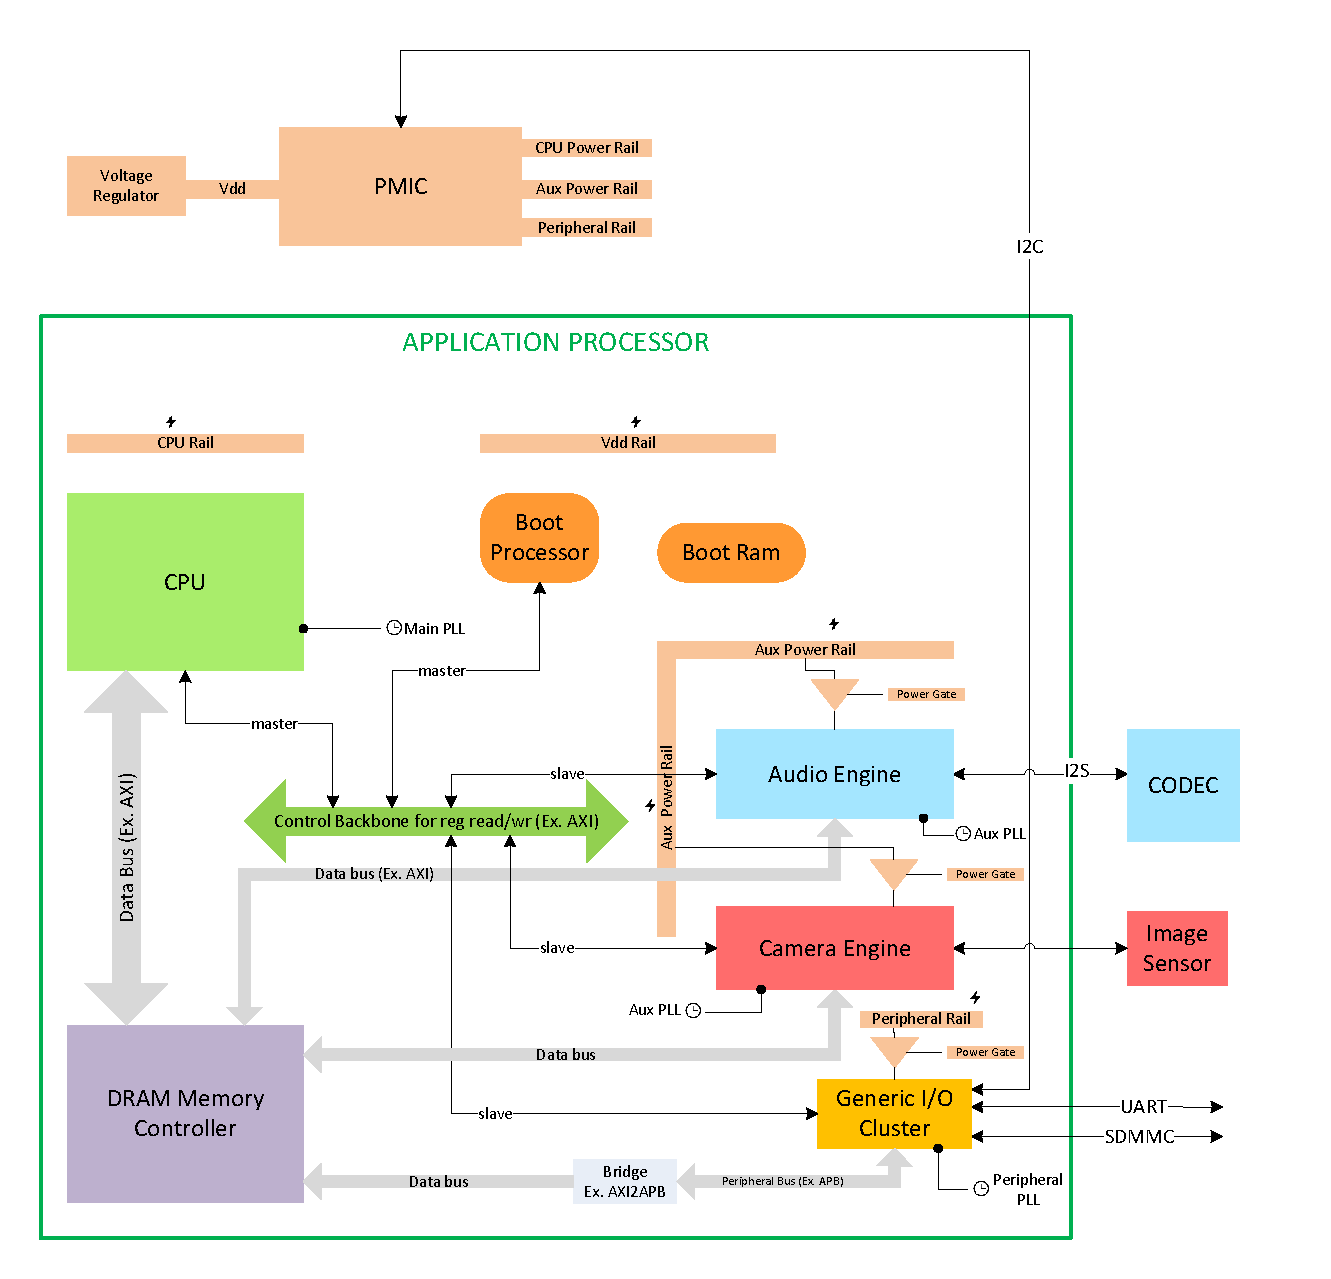
\includegraphics[width = \textwidth]{partSys/GenericApplicationProcessor}
	\caption{A typical Application Processor}
	\label{fig:genericAP}
	\end{figure}

A generic application processor (AP) consists of a CPU, Memory Controller (MC), I/Os, and, typically, many auxiliary engines. There could be multiple power rails supplying power at different voltage levels to different parts of an AP. Similarly there could be multiple clocks supplying clocks of different frequencies to different parts of the AP. 
	
The power rails are all connected to outputs of a Power Management IC (PMIC), which regulates the mains/battery power (a.k.a. Vdd) and has internal mechanisms to divide the regulated mains power to achieve the different power levels required on different power rails. A single power rail could be powering multiple blocks, each containing a ``power gate'' that can essentially turn that block on or off. \marginnote{Power rail levels, power gates can be used to control static power consumption}The power rails and power gates together give the voltage control granularity required to reduce the power consumption of the AP to the most optimal value. The PMIC itself is controlled via an I2C from the AP. 

The PLLs take reference clock from a crystal oscillator and generate integer/non-integer multiples of that clock.  Typically, one PLL output is used by several modules, each having a clock divider. These dividers are usually integer dividers or, integer.5 dividers (2, 2.5, 3, 3.5 etc.). Together, the PLLs and the dividers form the ``clock tree'' of the chip. The clocks going modules can be gated at many levels\marginnote{PLL output frequency, clock dividers, gates can be used to control dynamic power consumption}, including shutting down the entire PLL, primary gating, which gates one output of a PLL, second level clock gating, which is based on certain internal variables of a module indicating functional inactivity. All these can be used to optimize the power consumtion of the AP as a whole. 

The fabric (bus, like AXI) that the CPU uses to transact (read/write) data with the hardware registers of I/Os, hardware accelerators, PLLs etc., is called the ``Control Backbone''. This is usually different from the fabrics used by the CPU, auxiliary engines to transact data with the DRAM (via MC), which can be called the ``data paths''. The hardware register address space is colloquially referred to as, ``Memory Mapped I/O space'' or ``MMIO space''. So the Control Backbone is for accessing the MMIO space, while the data paths are used to access the DRAM address space. 

\section{A Note on Optimizing Power Consumption}
Optimizing power consumption is an important goal of a system architecture, especially if the system is expected to run out of a battery instead of the mains. There are two components of power consumption in an IC: Dynamic and Static power. Dynamic power consumption is because of loss when transistors toggle and Static power consumption is because of leakage from Vcc to ground of a transistor. If a module needs to run at a higher clock frequency, it would require a higher voltage. The higher the clock frequency, the higher the dynamic power consumption for the same voltage. Similarly, the higher the voltage, the higher the static (a.k.a. leakage) power consumption for the same clock frequency. \marginnote{DVFS in kernel is responsible for optimizing power consmption}The OS kernel in CPU usually does dynamic voltage and frequency scaling (DVFS) wherein it uses all the power, clock knobs described in the previous paragraphs to achieve the most optimal power consumption possible for a given use case. 
 
\chapter{Virtualization}
\label{chap:virtualization}
In general purpose systems, it is advisable to ensure that different processes or threads running on the CPU do not have visibility into each others stack, heap, global variables etc. This is to prevent malicious code from compromising other processes. Besides this, it is also advisable for each process to use virtual addresses instead of physical addresses for all memory accesses. This is to ensure that processes can be loaded into different physical addresses from one time to another and also to give processes a continguous address map while in reality the various addresses accessed by processes may be fragmented in the physical memory. \marginnote{OS gives virtual addresses to processes; does virtual to physical address mapping}The OS acts as an abstraction layer to achieve the above mentioned objectives, the umbrella term for which is \emph{virtualization} or \emph{software isolation}. One can extrapolate the concept of virtualization to running multiple OSs on the CPU at the same time (with each running their own pool of processes), wherein, another abstraction layer called a \emph{hypervisor} acts like a OS for OSs - One can think of a hypervisor as an operating system which schedules, virtualizes processes like any other operating system, just that for a hypervisor, a process is actually an OS with a pool of processes. People generally refer to this as many ``guest'' OSs running on a hypervisor. The necessity for having software isolation in a hypervisor case is exactly the same as that in the case of an OS. From here on, we will just talk about systems without hypervisor. One can easily extrapolate concepts below for the case of a hypervisor.
	\begin{figure}[h]
		\centering
		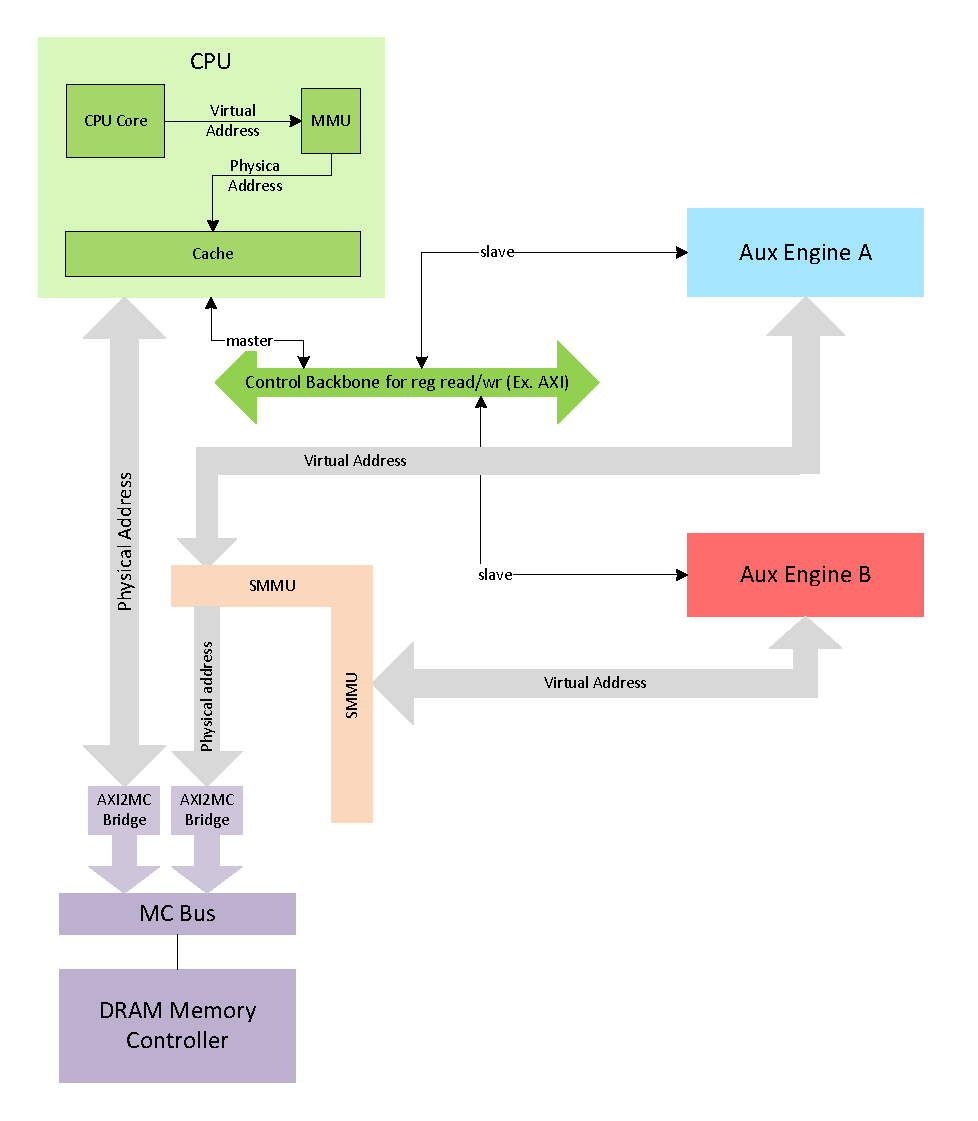
\includegraphics[width = \textwidth]{partSys/Virtualization}
		\caption{Virtualizaton in an Application Processor}
		\label{fig:virtualization}
	\end{figure}

\section{Page Tables}
The way an OS achives virtualization is by using \emph{page tables}. When a program is compiled and linked, the resulting \emph{elf}, \emph{bin} or \emph{hex} file contains, besides the code itself, some information about the program embedded in it. This information pertains to the size of code, size of the stack, global variables etc. When the program is requested to be executed, the OS looks into this information, allocates the require amount of memory (which aren't necessarily contiguous). Then the OS creates a look-up table, called the ``page table''\marginnote{Page table contains virtual to physical address mapping} that has the physical addresses of the just allocated blocks in one column and a corresponding set of virtual addresses in another column . Even though the physical addresses may not be contiguous, the virtual addresses always are. 

The page tables themselves are usually stored somewhere in the RAM by the OS. Before a process is run, its page table is loaded into a hardware module called ``Memory Management Unit (MMU)''. \marginnote{Kernel writes page table to MMU. MMU does actual translation}MMU's job is to take the virtual address generated by the CPU core at its input, and converts it into the corresponding physical address at its output. In other words, thought the OS creates the page table, the actual run-time translation is carried out by the MMU. The MMU generates a page fault if a process (possibly malicious) tries to access a memory outside its allocated virtual address range. When a context switch happens from one process to another, the OS, after halting the first process and before starting the second process, changes the page table in the MMU from that of the first process to that of the second. This is an important part of the security architecture provided by virtualization. The page table switch in MMU can be only achieved by a task running with a high level of security privilege. The OS thus runs in this priveleged mode and other processes cannot even access the MMU registers required for changing page tables.

The virtualization architecture involving MMU as described above is a watered-down version of real-word virtualization architectures. Should the reader require in-depth information, please refer to the Cache \& MMU section in  \nameref{chap:upArch}.

\section{Hardware Virtualization}
So far, we have talked about virtualization only from the point of view of software codes accessing the memory. But in an application processor, many hardware modules also access the memory. Some examples are DMA engines managing data traffic of I/Os and auxiliary CPUs. If a malicious code accesses, say, a DMA engine, and uses the engine to access memory that it otherwise cannot (because MMU will prevent it), then security will be compromised. This may sound unlikely at first - Afterall, a user mode program cannot directly access any hardware, including a DMA engine and it has to go through the hardware's driver which is part of the OS. Furthermore, any program would do a malloc to get a buffer for the DMA. The malloc itself goes through the kernel and the kernel will ensure that the address allocated is within the range of that program's legal range. The base address returned would of course be a virtual address. When the DMA is setup by the program, it uses the DMA driver which translates the virtual address to the physical address and gives it to the DMA engine. So all in all, it may sound like security cannot be compromised by a malicious code by misusing a hardware module. However, while the driver may not be checking whether the size of the DMA buffer exceeds the legitimate address range of the program. Many other complex scenarios like this are possible. Hence it is importnat to have a degree of control over the addresses accessible by hardware modules as well. This is where an SMMU (System MMU) comes into picture. \marginnote{SMMU is for hw what MMU is for SW}SMMU is very similar to an MMU - just like MMU does a virtual to physical address mapping using page tables that are different for different user mode processes, the SMMU maintains a page table for every hardware MC bus master. Thus, the DMA driver will, instead of translating the virtual base address from the user mode program to a physical address, it will translate it to a different virtual address and give this to the DMA engine. 

\chapter{DVFS}
\label{chap:dvfs}
Dynamic Voltage and Frequency Scaling is essentially the mechanism used by a system to ensure different components of the system (and hence the entire system itself) are consuming power optimally. The data transaction capacity of buses and I/Os and the processing capacity of other hardware modules will depend on the clock frequency at which the module is operating. For instance, a 16-bit bus, if clocked at 1 MHz, cannot carry bits at a rate faster than 16 Mbps. Similarly, a filter module requiring 5 clocks to process one sample would require the clock frequency to be at a minimum of $fs*5$, where $fs$ is the sampling frequency of the signal. While this is said about the clock frequency, transistors cannot be asked to toggle at any clock frequency at a fixed $V_cc$. Because a trasistor's transfer function has decreasing magnitude response with increasing frequency, there would be a point in the clock frequency after which the transistor voltage will have to be increased so that its ouput can be differentiated as a 1 or a 0 by the following transistor. Thus, one can think of a series of voltages and an associated range of clock frequencies supported by each voltage level. DVFS is all about fixing the clock frequency of a module, and hence, the voltage of that module, for a given use case. 

It is normal for a hardware module to share a voltage rail with many other hardware modules. So, for a use case, the DVFS mechanism will choose a voltage level for a voltage rail to be the maximum of the voltage levels required for the different modules connected to the rail. The case for clock frequency is somewhat similar - one PLL may be supplying clock to many hardware modules and its output clock is chosen to be the maximum of all the clock frequencies required for different modules sourcing clock from it. There is, however, a small difference - usually every hardware module has a clock divider that divides the PLL clock to obtain the required clock. This is because clock dividers are cheap. Thus the DVFS has the choice of changing the clock divisor for a particular module instead changing the PLL output. Power dividers, on the other hand, aren't cheap - PMICs are generally costly and their cost increases with the no. of rails they can support. \marginnote{DVFS has fine degree of clock control, coarse voltage control}So it is normal that DVFS has a fine degree of control over the clock frequency, but a much coarser degree of control over the voltage of a module.

\section{Synthesis Options for a Module}
In the first paragraph of this section, it was mentioned that a transistor has a transfer function that has decreasing magnitude response for increasing frequency. While this is true, it is not necessary for the entire chip to be made of the same type of transistor with the same transfer functiion - one can choose to synthesize one module with a particular type of transistor and another module with a different type of transistor. Usually transistors are broadly classified into different ``cell types'', such as HVT, SVT, LVT cells. The SVT cells can run at higher clock frequencies for a given Vcc than the HVT cells and the LVT cells can run at an even higher clock frequency for that $V_cc$. However, the penalty for choosing to synthesize a module at SVT, rather than HVT, is leakage power - SVT cells leak more than HVT cells (typically 25 - 65 times more). One may ask, ``what is the point of going to an SVT instead of an HVT''? SVT may require a smaller voltage for a given clock frequency as compared to a HVT, but it doesn't necessaily give us any power benefits as the leakage of SVT is higher than that of HVT. The answer for this question could be simple - it may be the case that the module in question is small in area and that we care more about the dynamic power consumption, which is directly proportional to the clock frequency, than its static power consumption, which is proportional to its area. However the answer could also be complex - the module in question may be connected to the same power rail as 10 other modules and, for a use case, the module in question may need a much higher clock frequency than all other modules under that power rail. Were we to synthesize the module in question at HVT cells, that would increase the rail voltage for 9 other modules. The collective power consumption (static+dynamic) in this case may be much higher than the case where the module in question is synthesized at SVT, and hence its higher clock frequency required doesn't push the rail voltage requirement up. \marginnote{Choosing right transistor for a module may involve module level, system level, use case level analysis}Of course, these calculation would vary wildly from one module to another, one use case to another. Beyond this, one needs to also consider the likelihood of the use case in question. Basically there is no single formula for choosing the cell type for a module. It is the job of the hardware architect to do the required analysis and prescribe the cell type of a module.

Besides choosing a cell type, one gets to also choose a finer granularity in transistor type. In other words, when a cell type is chosen, we would have only selected a class of transistors. Thus, even if we choose HVT as the cell type for a particular module, we still will have to choose, among all the transistors in the HVT class, which exact transistor to choose - within the HVT class, one can find one transistor to be capable of running at a slightly higher frequency at the same Vcc than a different transistor. Usually, it is very straightforward to choose the cell type for a module - normally CPUs would required faster cell types than, say, I/Os. The real job of the hardware architect then is to choose the correct transistor type within the selected cell type. 

\section{Real Life Methodology Used for Synthesis}
The above paragraphs may lead you to believe that the HW architect chooses the transistor type for a module directly. However the reality is different. Usually the hardware engineer first determines, among a set of use cases, which ones should be ``low voltage(LV)'' use cases, which ones should be ``medium voltage(MV)'' and which ones should be ``high voltage(HV)''. For example, a 16KHz stereo music playback (without video) may be determined as a low voltage use case, while a movie playback with 5.1 audio at 96 KHz may be chosen as a high voltage use case. After determining the ``voltage type'' of the use case, say LV, for every module that is run for that use case, the clock frequency at which it needs to run for that use case is noted as the ``LV corner'' frequency for that module. Thus, after classifying all the use cases into different voltage types and devolving the voltage type on the modules run during those use cases, we would have a ``LV corner'', ``SV corner'' and an ``HV corner'' (frequency values) for every module. This then is fed to the synthesis tool. The synthesis tool takes the preferred cell type as an input and selects the appropriate transistor type within that cell type for a module based on it LV, SV, HV corners - it basically chooses the transistor that will give the best power consumption based on these corner frequencies. If the synthesis tool cannot find a transistor type that satisfies the given corners for the preferred cell type, it will ask the user to choose a different cell type. So one starts with HVT cells and if the synthesis tool gives up, moves to SVT cells and so on. Remember that, with changing IC process (nm technology), the leakage characteristics of different cells and different transistors within the cell change - so it is humanly impossible for a hardware architect to manuall choose the transistor type for a module. Hence, synthesis tools are utilized to do the actual selection.


\chapter{Microprocessor Architecture}
\label{chap:upArch}
\section{Cache and MMU}
\emph{Cache} is a RAM that CPU has dedicated access to and which is used to temporarily store copies of data in main memory. The basic idea of a Cache is described in \nameref{chap:partHwMisc} chapter (part: Hardware), section ``Memory''. Here we assume the reader knows the idea and purpose of caches and focus on topics such as the working mechanism of cache, architectural options etc.

\subsection{Basic Cache Operation}
When a CPU issues an address for a read operation, the \emph{cache controller} checks if a copy of the data in that address (in the main memory) is available in the cache. If it is, then we have a \emph{cache hit} and the cache controller simply gives that data to the CPU without the need to actually fetch the data all the way form the main memory. If a copy of that data isn't available in the cache, then we have a \emph{cache miss} and the cache controller fetches the data from the main memory, gives it to the CPU and also store the data in the cache, so that, the next time CPU accesses the same address, we will have a cache hit. This is how data frequently accessed by the CPU (within the context of a function or a bunch of functions) build up in the cache resulting in less and less cache misses, and proportionally less accesses to the main memory. 
 
Compilers usually allocate memory contiguously for variables inside a function. And a function that is accessing a local variable one cycle is most likely to access another local variable within the next few cycles. So it make sense that, if a cache miss happens when the first variable is asked for, we fetch not just that variable, but also data from nearby addresses which likely belong to other variables that are soon to be accessed as well. This will reduce the likelihood of cache misses overall. A key idea here is that, while CPU is consuming the first variable, the cache controller is fetching the nearby address in parallel. And just as the CPU finishes consuming the first varaible and issues an access for nearby variables, we already have them in the cache. The amount of data fetched by a cache when a cache miss happens constitute what is called a \emph{cache line}. 
 
Let us take an example cache of 4KB size that serves a main memory of 4GB and see how the operations described above would work in this case. 
	\begin{figure}[h]
		\centering
		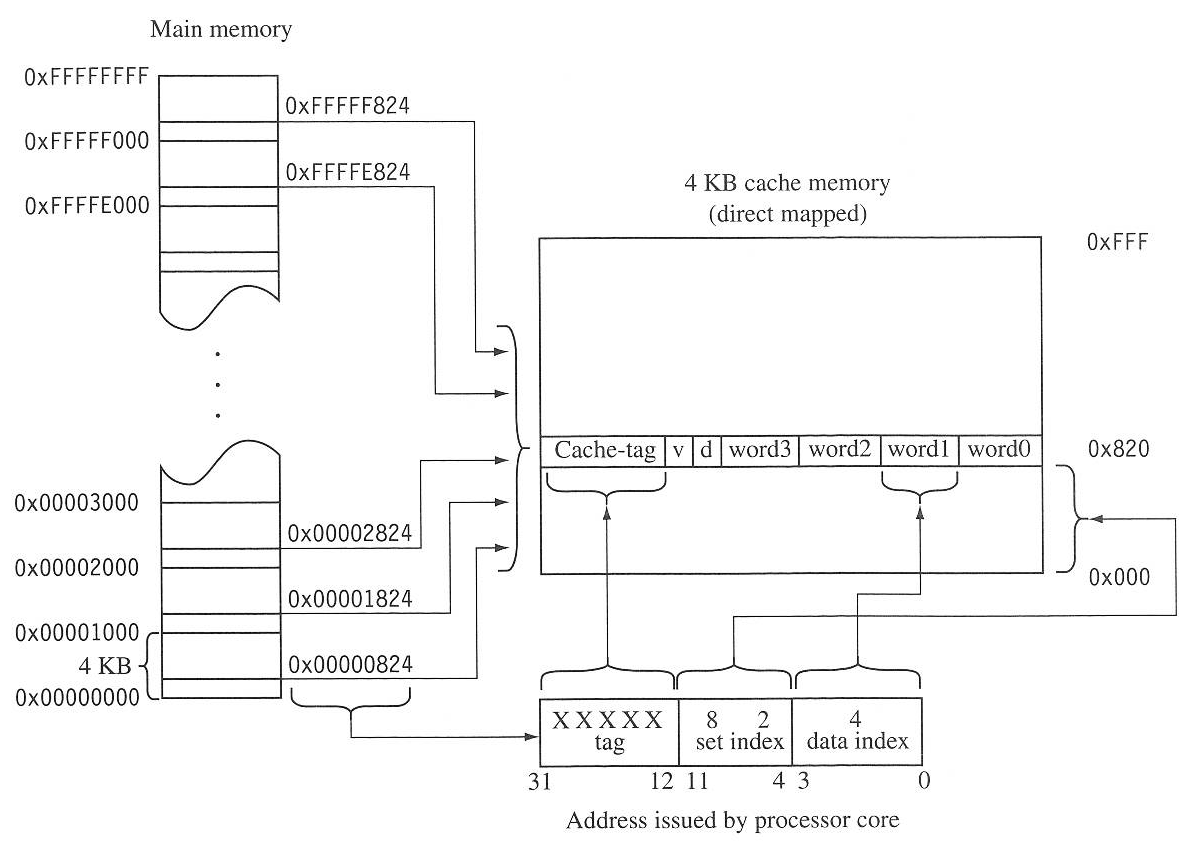
\includegraphics[width = \textwidth]{partSys/directMappedCache}
		\caption{Basic Cache Operation}
		\label{fig:basicCacheOp}
	\end{figure}
Mapping the 4GB address of the main memory to the 4KB address of the cache means that several addresses in the main memory will inevitably overlap in the cache. One way to do this is to simply divide the main memory into chunks of 4KB each and let them all overlap in the cache - this is equivalent to using only the least-significant 12 bits of the address issues by the CPU. Our example here uses this method. When the CPU issues a memory access, the cache controller initially ignores the most-significant 10 bits and uses the remaining 12 bits to look inside the cache (12 bits address equals 4kB, which is the cache size. So we are good). But when it reaches the cache line in that 12-bit address, it checks its \emph{cache-tag} which contains the most-significant 10-bits of the main memory address to which the data in that cache line belongs to. So the cache controller checks the cache-tag and if the cache-tag does match the most-significant 10-bits of the address issued by the CPU, we have a cache hit. Otherwise we have a cache miss. If a cache miss happens, the cache controller will feltch, in our example case, 4-words of data within the same 4-word-boundary as the address issues by the CPU from the main memory\footnote{Note that the cache controller will fetch the data in the address issued by the CPU first and only then fetch the rest of the data within the same 4-word-boundary, no matter where the CPU issued address is within that 4-word-boudnary}. The data thus fetched will replace the data in the cache line and the cache-tag will be promptly updated to contain the 10 MSBs of the address issued by the CPU.

Note that, in our example, instead of the cache controller looking for the LSB 12 bits of the address in one shot, it uses an 8-bit \emph{set index} first, looks up the cache line associated with it, check the cache-tag and only if there is a cache hit, will go look into the exact word within that line (or the 4 LSBs of the address). The idea of a set index is a natural consequence of the size of the cache line - when you know that the cache always picks up 4 words of data in one shot, then there is no meaning in checking if the exact word being asked is available - for it will be available as long as we have a cache hit for the entire 4-word-boundary.

So far, we have talked about how cache works for a CPU read. But a cache is also used for a CPU write - as much as we want to reduce the read traffic to the main memory from the CPU, so much we want to reduce the write traffic to the main memory as well. Imagine a scenario where a function running in the CPU reads a variable - we have seen how the copy of the data associated iwth this variable's address in the main memory will be made available in the cache. But what happens when the function manipulates that variable - there will be a CPU write and the data in the cache will be changed. Now the data value of the variable in the cache and in the data memory are different! Does that present us with a problem? Not necessarily and not right-away. As long as no other component of the system (a hardware accelerator or a DMA engine) is not accessing the same address location (of the variable in question), we are OK. If it is only the CPU that is going to continue to use that variable, further read accesses to that variable will only use the data in the cache, which is anyway fresh. However if the scenario is about to change - that a hardware accelerator now needs access to the new value of that variable, the CPU will have to issue a \emph{cache flush}. A cache flush is meant to write back the updated values in the cache to the main memory. But how does the cache controller know which of the values in the cache were updated by the CPU and which ones weren't? - it doesn't make sense to write back all the values in the cache to the main memory because that would be such a waste of bus bandwidth. This situation is tackled using the \emph{dirty bit} indicated by the letter ``d'' in the above \hyperref[fig:basicCacheOp]{diagram}. This bit is set everytime a word associated with the respective cache line is written to by the CPU. So when a cache flush is issued, the cache controller only writes back the cache lines that have this bit set.

The \emph{validity bit} is used for the exact opposite purpose as the dirty bit - Imagine a case when some component in the system, say a DMA controller associated with an I/O, writes into the main memory. Let us assume that the cache controller had acquired a copy of the data in that address location into the cache some time back. This means that the data in the cache is now stale and needs to be updated with the fresh data from the main memory. In this case, the CPU invalidates the cache \footnote{let us assume CPU came to know about the DMA writing into the main memory via a DMA completion interrupt}, i.e., sets the ``v'' bit to zero. And when the CPU access the invalidated address locations the next time, cache controller fetches data from the main memory instead of giving the stale data to the CPU. Again, notice that, just as in the case of the CPU read, we are note interested in updating all the invalidated cache locations with fresh data - that would be wasteful of bus bandwidth - but only those which are later accessed by the CPU. 

This section is under construction. Key words: Cache line (with valid and dirty bit), set association, cache, TLB architecture - \url{http://www.cs.cornell.edu/courses/cs3410/2012sp/lecture/22-vm3-i.pdf}

\section{Memory Management Unit}
This section is under construction. It will contain information on TLBs, what happens in MMU during context switching etc. 

\section{Fabric}
Even the most basic application processor will at least contain a CPU, a DMA engine, a Memory Controller and some I/O Controllers (if not any hardware accelerators). The way these talk to each other is through a fabric: Essentially AXI, APB, AHB, PCIE interfaces from these modules go to a interconnect switch which arbitrates, routes communication between pairs of interfaces. CPU and the DMA engine, in our example, will be Masters on the interconnect, whereas the Memory Controller and I/O Controllers will be slaves. Only the masters can initiate a communication (mem read/write, reg read/write) and the slaves can only respond. The traffic in the fabric can be broadly classified into MMIO access (basically register read/write) and Memory access (basically DRAM or some SRAM). The masters have different priorities. In case two masters try to access the same slave at the same time, based on their priority level and possibly the traffic type (and may be even some other parameters), the inconnect switch will decide which master will get the link to the slave. 

\subsection{Switch}
Let us take a simple Application Processor as shown below. Let us use this as an example to explore the functionality of a switch in detail. 
	\begin{figure}[h]
		\centering
		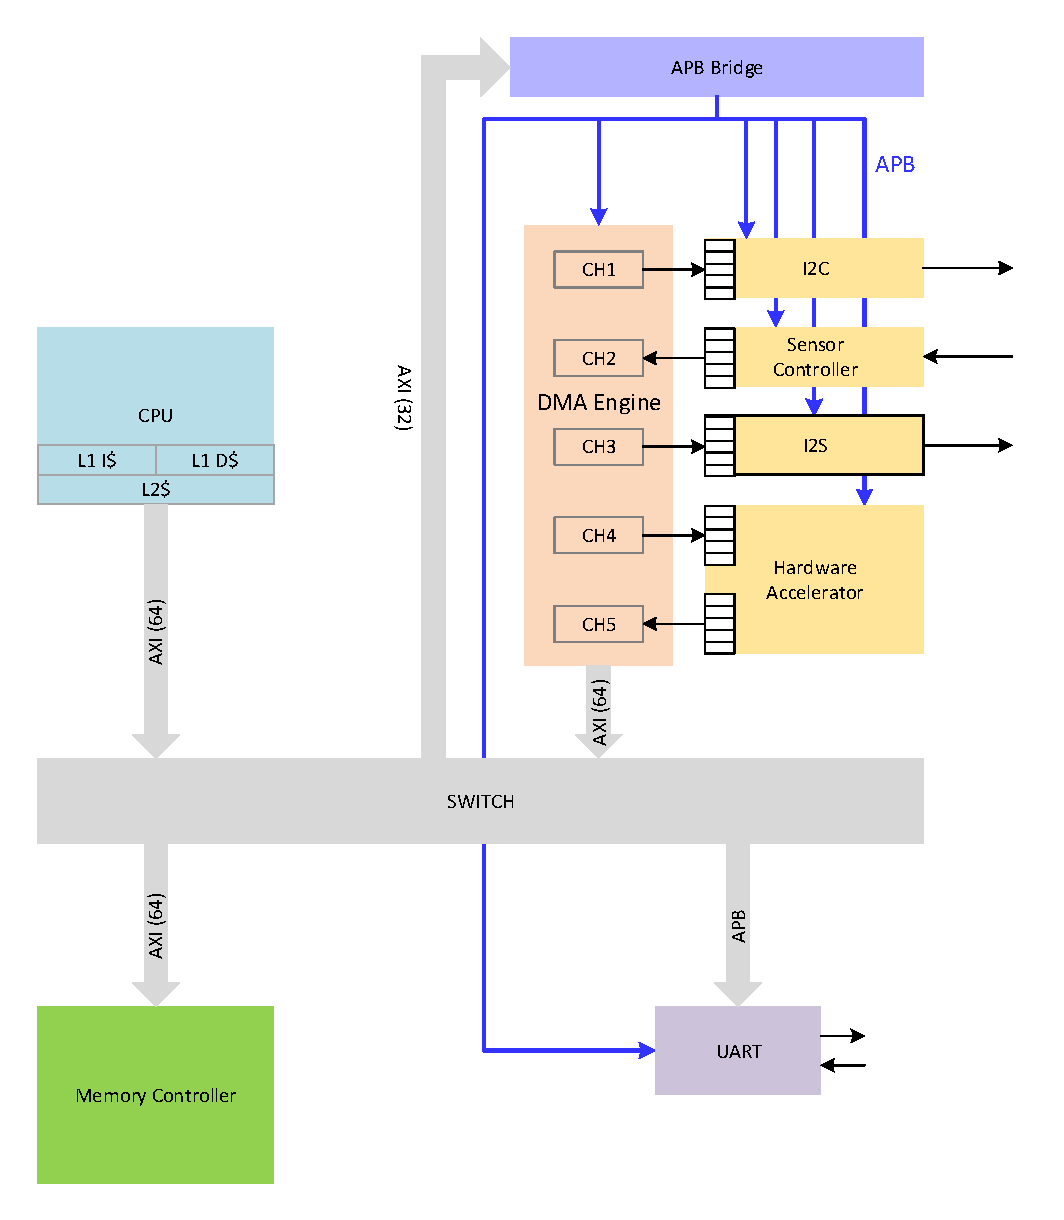
\includegraphics[width = 0.5\textwidth]{partSys/SimplestAP}
		\caption{A Simple Application Processor}
		\label{fig:simpleAP}
	\end{figure}

Basically the CPU can access the system memory via an AXI and configure the rest of the hardware (MMIO space) in the system using an APB multi-port Bridge \footnote{An APB Multi-port, uses a single APB bus connecting all the hardware (all the hardware module's basically evesdrop on the bus's signals) and the APB Bridge drives the signals on the line (seen by all hardware), but raises the chip select of only one of them. This way we can avoid having each hardware hooked up to an independent APB bus which will increase the wire count of the system.}.  The DMA engine (DMAe) supplies data from the system memory to I/Os and hardware accelerators without CPU having to read data and write to the hardware one-by-one (with data FIFOs of hw sitting in the MMIO space). 

Now the switch has two functionalities: Arbitration and routing. Let us assume that CPU has higher priority that DMAe - so the arbitration in our simple AP case is...well simple. Next, to know which slave to route a master's request, we need to deal with the important concept of the \emph{Address Map}. But before we go into the Address Map, we need to remember a key point: The masters have no idea in which slave a memory address is located. So their read/write requests only contain the destination address and the destination slave - It is entirely the job of the switch to figure out which slave a request should be routed to.

Address Map is simply a division or allocation of available addresses in the system to various slaves. Let us say that we decide that the system address will be 32-bits wide \footnote{Address width is determined at architecture time. It doesn't have to be a power of two. 37-bit, 26-bit address widths are not unusual}. This means that the AXI buses coming out of masters and going to slaves will have 32-bit wide address signal. Anyway, this 32-bit address width implies a 4GB address space. Let as assume that (for whatever reason), we decide on the following address map.

	\begin{figure}[h]
	\centering
	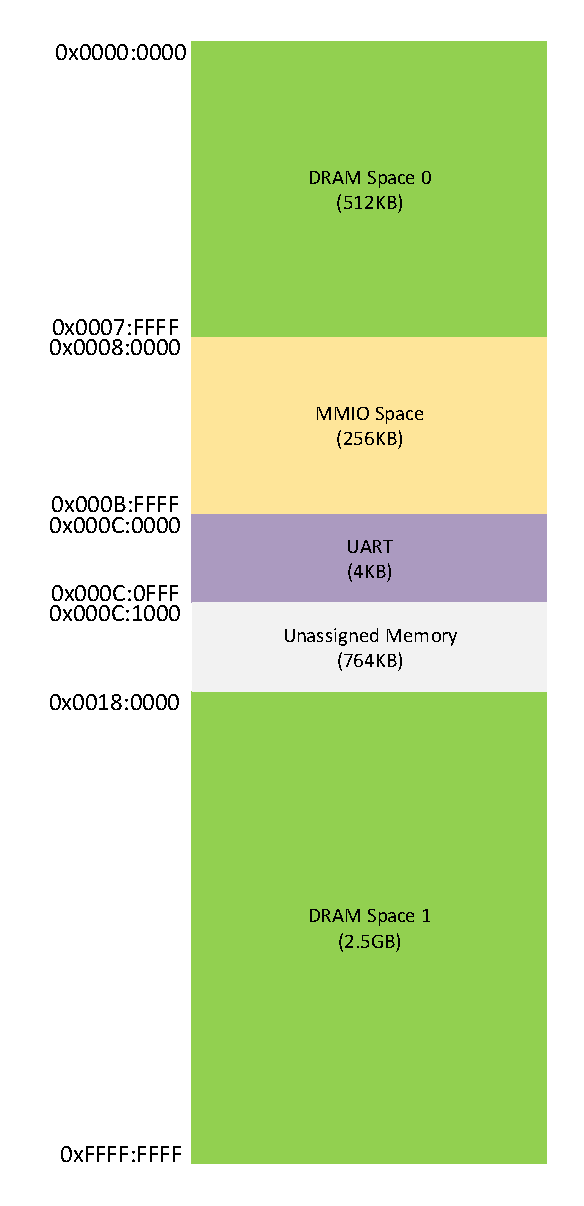
\includegraphics[width = 0.5\textwidth]{partSys/Amap}
	\caption{An Example Address Map}
	\label{fig:sampleAmap}
	\end{figure}
	
Thus DRAM gets two address \emph{apertures}\footnote{An aperture in an AMAP refers to a contiguous range of addresses}, while MMIO and UART get one aperture each. This address map is known to all the masters as well as the switch itself. So, for instance, the CPU (OS) knows that data memory is either in DRAM space 0 or 1 and hence allocates stack and heap only in those areas. And the switch uses the address map to figure out to which slave it should forward a master's request to based on the destination address bits in that request. 

The switch considers all the addresses within the address map to be legitimate unless the address map explicitly mentions an area as unassigned (as in our example). In the case of the master's request containing an invalid (unassigned) address, the switch will respond with an address decode error. Otherwise it will forward the request to the next level, which can be a bridge (like the APB Bridge) or a end client itself. Now it is the responsibility of the bridge or the client to tell the master if an address is illegitimate: Even if the address map shows a contiguous MMIO space, it may have large unassigned address ranges within it. In fact, even going further, a module that occupies a set of addresses within the MMIO region may have empty space it reserved for future expansion. In the former case, the APB Bridge (in our example, that is the only MMIO master on the MMIO APB bus) will respond with decode error. In the latter case, the end module will. 

One may wonder why the DRAM space is split into two apertures. Though it was done just to let the reader know that one slave can have two apertures assigned to it, it isn't uncommon to find such an arrangement in real-life systems. The reason is that, some CPU, for security reasons, don't allow accesses beyond 1GB (or some arbitrary value) of address space during boot time. So it becomes necessary to put all the addresses one may need during boot time within the 1GB.

The address map tells the switch to which slave a master's request should be forwarded to. However, it doesn't tell the switch whether to forward that request at all or deny access. Often it is useful to have switches restrict access of certain masters to certain slaves for security reasons. For instance, the system architect knows that the DMA Engine has no business accessing the MMIO space. So s/he may want to switch to not allow a DMAe request to be forwarded to the APB bridge even thought that request contained a legitimate address according to the address map. This is because hackers could exploit an unrestricted access and use DMAe to make a chip to hang.

These address restrictions are encoded in a \emph{Connectivity Matrix} as shown below

	\begin{table}[h]
	\arrStr{1.3}
	\begin{tabular}{l l l l}
	\toprule
	Connectivity (MxS) & Memory Controller & APB Slave & UART\\
	\midrule
	CPU & {\color{green} Yes} & {\color{green} Yes} & {\color{green} Yes}\\
	DMAe & {\color{green} Yes} & {\color{red} No} & {\color{red} No}\\
	\bottomrule
	\end{tabular}
	\caption{Connectivity Matrix}
	\end{table}
	

\section{Issues Relevant to Fabrics}
\subsection{Access Restrictions}
Access restrictions don't stop with the connectivity matrix of a switch in a Fabric. It only gives an extremely coarse level of restriction. It is possible that we don't want a slave to be accessed by master at some times, but not at other times. For ex., we don't want hackers to overwrite some program memory area - In this case unless the CPU master's access originated in the SW from the OS (and not user's code, which could be hacker's code), we should not grant it access to certain memory areas. Going even further, we may want another level of security, whether, even if the access was generated by OS, if it was not in a secure mode (like ARM's Trust Zone mode), we may not want to grant access to, say, the region in DRAM that stores digital signatures, private keys etc. These additional levels are restrictions are implemented not in the switch, but in the slaves themselves. AXI protocol has three \emph{PROT} bits that are set by the master depending on which mode the SW that generated the request was in. In DRAM, there could be a bunch of address (sub)apertures that have different levels of access restrictions implemented: DRAM may grant access to some apertures only if the PROT bits indicate a secure access, and some to secure or privileged access etc.

While the PROT bits are native to the AXI protocol, it is possible that the system architect may want a different type of security. For ex., s/he may want to DRAM to differentiate between a privileged access coming from a certain master from the privileged access coming from certain other master. In this case, though AXI won't support it natively, s/he can use AXI's generic \emph{user bits} (AWUSER). This can be made to carry, say a 4-bit custom master ID - In hardware, at the AXI interface between a master and the switch, the wires associated with user bits can be pulled up or pulled down to create a master ID pattern that is essentially hardwired into the system (and hence impossible to defeat).

\subsection{Latency}
Latency is the delay seen by a master from when it puts out a request to when it gets back a response. Imagine a human interaction situation in which a news anchor is talking, over a satellite connection to a field reporter. We often see that it takes several seconds for the news anchor's questions to reach the field reporter. And the field reporter processes the question in her brain and replies. Similary in a network, when a master puts out a request, it may be delayed due to arbitration at the switch(es), arbitration at the slave and also slave request processing time. In the human interaction example, to tackle the latency, the best strategy is for the news anchor to ask many questions in a row - so while it takes some time for the first question to reach the field reporter, she can process several questions in a row and offer a lenghthy response. This strategy works as long as the news anchor's one question doesn't depend on the field reporter's answer to his previous question. This plays out the same way in a network. Thus, as long as requests are independent from one another, the master may choose to send many of them back to back instead of sending each request only after the previous request received a response. 

In our example AP, the DMAe has to provide the I2S samples isochronously so that the I2S never runs out of samples to send out to the external world. Imagine that the data rate of the I2S is 48KHz and its samples' size is 32-bit. Let us also assume that DRAM word size is 32-bits as well to make this illustration simpler. Let us assume that the bus protocol or DRAM restriction allows a single request to upto 16 words and no more (i.e., a single, say, AXI request can indicate that it wants 16 words of data). And let us assume that the network max latency is 1ms. For simplicity, let us further assume that the DMAe has a big FIFO in each of its channels and that the I2S has no FIFO of its own. In this case, a good strategy for the DMAe would be to first make a 1ms worth of requests every time its internal memory is touches a lower limit of 1ms worth of samples. In other words, at the very beginning, the DMAe would make three requests, each for 16 words to the DRAM (3*16 = 48 samples = 1ms worth of samples). Now when it receives back-to-back responses from the DRAM, it fills its internal buffer with these responses, i.e., 48 samples. But immediately this value is at the lower limit level of 48 samples. So as soon as it receives all the responses from the DRAM, it makes another three 16-word requests. Suppose this second set of requests get their response within 0.5 seconds (since 1ms is only max latency), its buffer will now contain 1.5ms worth of data (I2S drained 0.5ms of data in the mean time..). This time, the DMAe doesn't have to make its third set of three 16-word requests right after it got the back-to-back responses from the DRAM. It can wait for 0.5ms (at which point, its FIFO will have 48 samples left) and make the next set of requests. 

Remember that, in AXI, the request channels and response channels are completely independent. So the fabric can absorb requests coming from a master (by raising `ready' signal) into an internal FIFO somewhere (and then forward the request to the slave when its time comes), but not respond. Think of it as packets in a computer network: When the home computer makes a request to the google server, those packets are accepted right away by the switch and then by routers, but only the google server responds - the switch or router don't. And while the packets to google server are in transit, the home user can make a separate request to some other site without waiting for google server's response.

Coming back to our DMAe's strategy of sending out 3 requests in a row, this means that somewhere in the fabric, the DMAe must have for it 3 requests worth of buffer available. This could be at the point where the DMAe connects to the switch or the point where the switch interface to the DRAM originates. In the former case, we could simply have a 3-request buffer. In the latter case, since other masters would also be accessing DRAM, the buffer needs to account for DRAM as well as other masters. This concept of multiple back-to-back requests is called, ``maximum outstanding requests''

\subsection{Ordering OOO replies}
Memory Controller, as a rule of thumb, never responds in the same order in which it received requests causing the phenomenon of \emph{Out of Order replies}. This is because, it sees that the earliest arrived request requires it to open a new memory bank that the one that is already open, whereas a later arrived request is to the already-open memory bank. Frequently switching between memory banks is wasteful of power and also has latency implications. 

For some masters, in some cases, it is OK to receive OOO replies. For example, a DMAe requires all requests originating from a particular channel be responded to in order - but it doesn't require, say, two requests coming from two different channels be responded to in order. Thus we need some way of differentiating between the set of requests that require in-order responses and those which don't care. In our example AP, the fabric uses AXI IDs (AWID field) - requests that have the same AXI ID need responses in order. But requests that have different AXI IDs can be responded to OOO.

At this point, it is a good idea to understand the idea of AXI IDs a little more. 
	\begin{itemize}
	\item AXI IDs are not associated with masters and are associated with transactions, but are not necessarily associated with slaves. So two requests going to the same slave could have two different AXI IDs. 
	\item One master can use multiple AXI IDs. But the method used by a master that determines what AXI ID to use for a particular request is completely up to the master and is implementation specific
		\begin{itemize}
		\item For ex., a DMAe can be implemented to use one AXI ID for each of its channels. A CPU can decide to use one AXI ID per thread.
		\item A master may choose to use different AXI IDs for different slaves. But this is matter of strategy and hence doens't negate the top point in this list. An example is to avoid head-of-line blocking of requests associated with fast slaves by requests associated with slow slaves. More about this can be found in later subsections.
		\end{itemize}
	\item Two masters cannot have use the same AXI ID. AXI IDs are thus allocated by the system architect to different masters - Some masters may get many. Some may get few. Some may even get just one AXI ID.
	\end{itemize}
	
Coming back to OOO replies, it becomes the responsibility of the fabric to re-order OOO replies from the Memory Controller for requests that require in-order responses. So the fabric has to do some sort of book keeping of (AXI ID, destination address) pairs (near the point where the AXI to slave goes from the switch) and when the replies come from the MC, re-order as necessary.

\subsection{Head-of-Line Blocking}
Head-of-line blocking is a generic term which means that a head item in a FIFO is in someway restricing an item behind it in the queue. A human interaction example would be when a driver is waiting at the intersection in a single lane (one lane on both sides) road to make a right turn (i.e. in India). He needs to wait for the opposite side traffic to have a moment of pause before he makes a turn. But because it is a single lane road, all the drivers behind him have to wait for him to make the move, even though the others are thru traffic - In other words, even though the way is clear for most drivers, they still can't move because the way isn't clear for the head driver in the queue. 

The following scenerios of head-of-line blocking issue are common in fabrics.
	\begin{itemize}
	\item A master's request to a readily available slave is waiting because another to non-available slave is blocking it at the head of the queue
	\item A CPU thread is blocked at the head of the queue by a non-available slave, but other threads accessing other slaves get their requests blocked behind the blocked thread's
	\item CPU requests to fast responding slaves is blocked by requests to slow responding slaves (with all the switch buffers for outstanding requests filled by requests to slow slaves)
	\end{itemize}

The strategy for tackling head-of-line blocking involves the clever use of AXI IDs (as we did with OOO replies earlier). At the master side of the switch, one could have different sets of outstanding request FIFOs for different AXI IDs. \footnote{``sets'' of FIFOs, because AXI has 5 channel and supporting, say 4 outstanding requests, means having not one 4-deep FIFO, but 5 4-deep FIFOs - i.e., one FIFO for each channel}. Basically our strategy of unblocking the queue is not to have a single queue in the first place! i.e., have different queues for different AXI IDs. So the afore mentined scenarios can be resolved using the following AXI ID allocation strategy respectively.
	\begin{itemize}
	\item Use different AXI IDs for different slaves
	\item Use different AXI IDs for different threads
	\item Use one AXI ID for fast slaves and one for slow slaves
	\end{itemize}
	
Of course, it is not possible to give one set of FIFOs for each AXI ID if the no. of AXI IDs used by a master is too many. So the system architect judiciously decides on how many sets of FIFOs to give to a certain master, and which AXI IDs go to which FIFO (so several AXI IDs could go to the same FIFO). 
	
\chapter{Miscellaneous}
\label{chap:partSysMisc}
\section{Coherency}
When there are many processors in a system (think of a CPU cluster with 4 CPUs), each CPU will have its own (L1) cache containing independent sets of cache lines. But if one CPU updates a cache line and then a second CPU accesses the physical memory corresponding to it, the coherency mechanism (hardware module) detecs that the second CPU is accessing stale memory. This coherency mechanism then does a cache flush of that cache line from the first CPU and also invalidates that cache line in the second CPU (so that it's cache DMA will automatically go fetch the freshly updated memory content). Note that, while each of the CPU cores will have its own L1 cache, there is usually an L2 cache shared by all the cores. So whena coherency needs to be done between two CPU cores, a L1 cache flush of one core doesn't necessarily have to update the physical memory in the DRAM, but could simply update the L2 cache. Exactly which method is used will depend on the architecture of the coherency mechanism

I/O coherency reference to something similar when a DMA is involved. If someone sets up a DMA to transfer data to an I/O from a mem location, if the DMA is I/O coherent with the CPU, it means the coherency mechanism will come to know that DMA is going to fetch from a memory location - and if that location is stale, it carries out a cache flush of the corresponding cache lines (which were recently updated) of the appropriate CPU. It works the other way around as well (in case DMA is sending samples from I/O to mem).

\section{Booting}
Booting is about setting up an application processor for loading the OS (kernel). In an application processor, either the main CPU or an auxiliary CPU can be used for booting - For now, let us assume that there will be a separate boot processor. At power up, the PMIC has the only the Vdd rail ON and other rails will be OFF. The PLL that supplies clock to the boot processor must be on the Vdd rail so that it can start supplying clock to the boot processor right after power up. The boot processor and the boot ROM that the processor executes data from need to be on Vdd as well. The first thing the boot code does is to power up (and enable clocks to) some local boot RAM, copy the rest of the boot ROM code on to that RAM and then execute the rest of the code from the RAM - Usually ROM r/w is pretty slow and this is why this step is done. After this point, the boot code turns on power rails, clocks, configure pinmuxes and do whatever is required to read from the bootloader medium. This may be an SD card. Thus the boot ROM only contains minimal code required to load the bootloader, which then takes care of rest of the boot loading. The rest of the boot loading is again about turning of power rails and clocks and configuring hardware registers in the appropriate sequence. The idea of the boot loader is to run some tests to ensure the hardware is OK and then to load the Linux Kernel on to the CPU. Eventually the Linux Kernel will load Android (or GNU). 


























